In this chapter the planning and work-flow regarding Sprint 4 will be described. 
Everything from setting our goals to implementation and testing. At the end we will evaluate the whole sprint and try on answer the following questions: What went well? What could be improved? 
\section{Sprint planning}

The customer was very satisfied with the demonstration video for sprint 3. Now we planned how to take the project further. At this point we were able to send control signals to multiple clients, and then detect the devices that lit up. We decided that the plan for this sprint was to combine those two, and try to create an image. We wanted to create a traffic light. This meant that after detection, we had to send signals to make the first client light up red, and make the second one light up yellow, and then make the last one light up green. Since the main goal was to make the mobile screens create an image, the order of the different colors was be imporant. We had to plan for making specific devices to light up specific colors at spesific positions. A traffic light was a good start for focusing on this part of the assignment, and the customer agreed. For sprint 4, the plan was to first map all available devices to grid, and then link the devices location with their ids, and then make the clients create a traffic light.  


In sprint 4 we also planned to work more on the report. Our plan was to finish sprint 3, since that sprint finished the week before. We also wanted to start working on sprint 4. Since we had implemented detection of devices, and we planned to link their location to their ids, we figured that we needed to add more information about the software architecture as well. We where also starting to get a better understanding of what the end product would look like, therefore we planned to also start working a little bit on the evaluation. The supervisor also came up with some suggestions for small improvements on the report, which we planned to work on. Also we needed to make to the user stories more consistent. We also planned to separate the implementation stories from the documentation, and the project management stories.

\subsection{Duration}
This sprint is 2 weeks long. From 14th of October 2013 to 27th of October 2013. We agreed
on the date of presentation and showing the running demo – on Thursday 25th of October 2013.
Estimated velocity is 240 hours since we agreed on 30 working hours per person per week.

\subsection{User-stories}
\subsubsection*{Implementation}
All the functional requirements for sprint 4 are presented in table \ref{tab:sprint4stories}
\LTXtable{\textwidth}{sprint4/stories.tex}

\subsubsection*{Documentation}
All the documentation stories for sprint 4 are presented in table \ref{tab:sprint4Documentationstories}
\LTXtable{\textwidth}{sprint4/storiesDocumentation.tex}

\subsubsection*{Project management}
All the project management for sprint 4 are presented in table \ref{tab:sprint4storiesProcess}
\LTXtable{\textwidth}{sprint4/storiesProcess.tex}

% hous all in total: Estimated: 130 + 65 + 42 = 237  Spent: 136+ 36+35= 207
\section{Preliminary studies}
% TODO
\section{Sprint goal}

The goal for sprint 4 is to link the devices location with their ids, and then make the clients create a traffic light together. 
\begin{figure}[H]
	\centering
		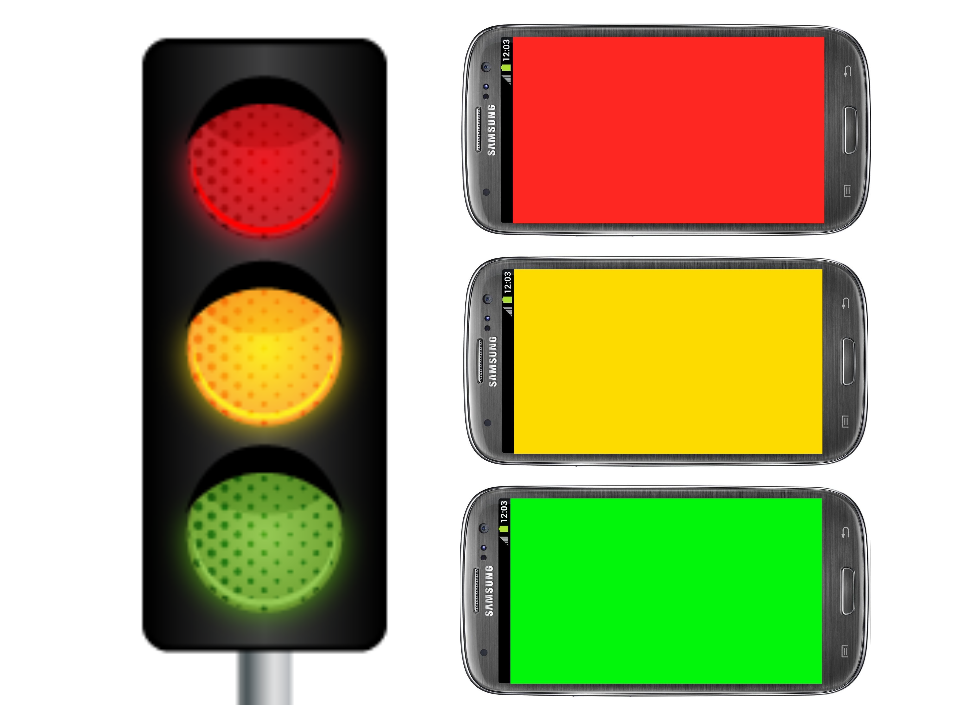
\includegraphics[width=10cm]{sprint4/trafficlight.png}
	\caption{Traffic Light.}
	\label{fig:trafficlight }
\end{figure}

\section{System Burndown}
\begin{figure}[H]
	\centering
		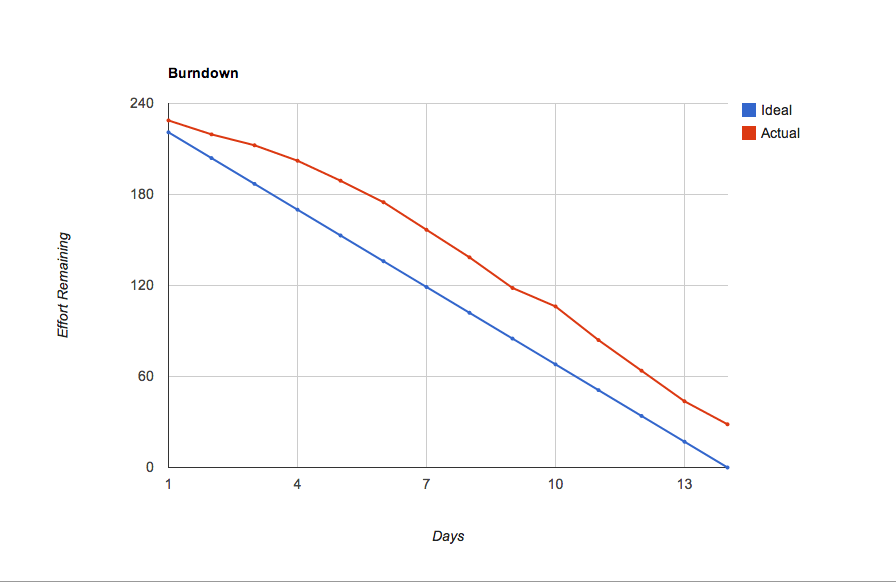
\includegraphics[width=18cm]{sprint4/BurndownSprint4.png}
	\caption{Burn down chart.}
	\label{fig:Burn4 }
\end{figure}
\section{Architecture}
\section{Implementation}
\section{Testing}
\section{Occurring risks}
\section{Customer feedback}
\section{Retrospective}
This section reflects on the past sprint. In order to learn from the mistakes done and thus to improve the workflow it is necessary to answer two essential questions: "What went well" and "What could be improved".

\subsection{What went well}
\subsection{What could be improved}
